\section{Introduction}

In Chapters 1 and 2, I presented a model of perceptual choice and showed it can systematically predict the repulsion effect, but not the attraction effect. In this chapter, I test another prediction of the model while demonstrating an important empirical result in another domain: best-worst choice.

\subsection{Introducing Best-Worst Choice}

Best-worst choice (also known as best-worst scaling) is an experimental paradigm where participants select their most and least preferred options from a choice set. Originally proposed by \textcite{finn1992determining}, best-worst choice is widely used in a number of applied fields, such as transportation \parencite{beck2016best} and healthcare economics \parencite{cheung2016using,flynn2007best}. One key advantage here, when compared to traditional discrete choice research, is that researchers can use best-worst choices to gain information about participants' ranking of options while never requiring them to complete a full ranking task, which may be quite difficult \parencite{marleyProbabilisticModelsBest2005}.

In addition to the empirical applications, researchers have developed theoretical results on best-worst choice, with many models relating best-worst choices to an underlying utility function. \textcite{marleyProbabilisticModelsBest2005} developed a class of models known as "maxdiff" (maximum difference) models of best-worst choice\footnote{Note that the term maxdiff is sometimes erroneously used to refer to best-worst experiments in the generic sense. Following \textcite{marleyProbabilisticModelsBest2005}, I use maxdiff to refer to a specific class and parameterization of choice model.}. According to the maxdiff model, given choice set $K$, the probability of selecting option $x$ as best and option $y$ as worst (where $x \neq y$) is defined\parencite{hawkinsIntegratingCognitiveProcess2014a}:

\begin{equation}
   BW_{K}(x,y)=\frac{e^[u_{x}-u_{y}]}{\sum_{\substack{{p,q}\in K\\p \neq q} e^[u_{p}-u_{q}]}}
   \label{maxdiff_equation}
\end{equation}

where $u_{i}$ is the utility of option $i$. This model proposes a single utility function that determines best and worst choices. Specifically, it proposes that best-choice probabilities are an increasing function of $u$, while worst-choice probabilities are a decreasing function of $u$. The use of the exponential function means that the maxdiff model is another form of the widely used multinomial logit (MNL) choice model \parencite{hausman1984specification}. Furthermore, so long as $u$ does not vary based on choice set, the maxdiff model predicts a monotonic relationship between best-choice probabilities and worst-choice probabilities.

There are many variations on this model \parencite{marleyProbabilisticModelsBest2005a,marleyProbabilisticModelsSetdependent2008,marleyModelsBestWorst2012,flynnBestWorstScaling2007,flynn2014best}, though the maxdiff model remains the dominant model for analyzing best-worst choice data.

Researchers have explored whether this monotonicity holds empirically. \textcite{hawkinsIntegratingCognitiveProcess2014a} examined both preferential and perceptual best-worst choice data using response time modeling. They used the linear ballistic accumulator model (LBA) \textcite{brownSimplestCompleteModel2008b}, which casts the decision process as a race between "accumulators" towards a threshold, where the average accumulation across trials is captured by the drift rate parameter. Modeling datasets containing both preferential and perceptual best-worst choice data, they were able to successfully account for choice data by assuming a parallel race between "best" and "worst" accumulators for each option. Furthermore, they showed that the utility values estimated for each option using a MNL model were positively linearly related to the log drift rate values from the LBA, suggesting an underlying utility representation that captures choices. 

In a follow-up \textcite{hawkinsBestTimesWorst2014} found that, collapsing across choice sets, best-choice probabilities are (negatively) monotonically related to worst-choice probabilities. They also showed that, using the parallel best-worst LBA as a model, the drift rate parameter for worst choice can be parameterized as the reciprocal of the best choice drift rate. Formally, if $d_{b}(i)$ is the drift rate for selecting option $i$ as best, then $d_{w}(i)=1/d_{b}(i)$, where $d_{w}(i)$ is option $i$'s drift rate for best choices. 

We can think of the parallel best-worst LBA as a process implementation of the maxdiff model \parencite{hawkinsIntegratingCognitiveProcess2014a}, which proposes set independence. While researchers have proposed models that allow set dependence \parencite{marleyProbabilisticModelsSetdependent2008}, these models still predict a monotonic relationship between best and worst choices. 

It is not always the case, however, that a single latent variable (i.e., utility) underlies choices. Indeed, as I show below, the model from Chapters 1 and 2 predicts, under certain conditions, a dissociation between best and worst choices.

\subsection{Model Predicted Dissociations Between Best Choices and Worst Choices}

Let $K$ be a choice set consistings of options $T$, $C$, and $D$ (i.e., target, competitor, and decoy). As in Experiments 1 and 2, these are rectangles in a perceptual choice experiment. As above, I asssume that on each trial $i$ with choice set $K$, The perception $\mathbf{X_i}$ of all 3 stimuli is sampled from a multivariate Gaussian distribution with a mean vector $\mathbf{\mu}$ and variance-covariance matrix $\mathbf{\Sigma}$ (see \ref{eqn:mvnorm}).

$\mathbf{\mu$ and $\mathbf{\Sigma$ are parameterized the same as in Chapters 1 and 2. 

In this chapter, I apply the model to best worst choice by assuming that, given a vector $X_{i}$ of perceived areas on trial $i$ with set $K$, the probability a participant selects stimulus $i$ is as best is:

\begin{align}
   P(i|K)=P(X_{i}>X_{j}, j \in K, i \neq j)
   \label{eqn:bchoice1}
\end{align}

while the probability of selecting stimulus $k$ as worst (where $i \neq k$) is:

\begin{align}
   P(k|K)=P(X_{k}<X_{j}, j \in K, k \neq j)
   \label{eqn:wchoice1}
\end{align}

As it happens, the correlations (i.e., $\Omega$) estimated from Experiment 2 predict that, in a best-worst choice paradigm, best and worst-choice probabilities are non-monotonically related. I demonstrate this using simulations.

To simulate best-worst choice, I simply used the mean parameters ($\mathbf{\mu$ and $\mathbf{\Sigma$) estimated from Experiment 2\footnote{I used only those estimated from the triangle condition (See Experiment 2).} and simulated a large ($N=10000$) number of choice trials. I collapse over choice set (as in previous reported simulations) and focus on target, competitor, and decoy choice proportions at each level of TDD. I show these results in figure \ref{fig:bw_sim}, in a state-trace plot \parencite{newell2008dimensions}. State-trace analyses plot the values of two dependent variables against each other for a particular experimental condition. State-trace analysis can be controversial \parencite{ashby2019state,ashby2022state,stephens2020state}, and statistical inference on state-trace data is not straightforward \parencite{sadil2018hierarchical,davis2016bayes}. In principle, however, if the analyst can reliably conclude that the data points do not fall on a single curve, they conclude that the data vary on at least $2$ dimensions.

\begin{figure}
   \caption{Best-worst choice simulations. Each row is a different TDD value from Experiment 2.}
   \label{fig:bw_sim}
\end{figure}

The model, conditioned on the estimated parameters, predicts an interesting result. Although the competitor is most frequently chosen as best, due to the repulsion effect from Experiment 2 and from \textcite{spektorWhenGoodLooks2018b}, it is not, however, least frequently chosen as worst. Specifically, $B(C)>B(T)>B(D)$, while $W(T)<W(C)<W(D)$, where $B(i)$ and $W(i)$ are the probabilities that option $i$ is chosen as best and worst, respectively.

The reason for this prediction is that because $\rho_{TD}>\rho_{CD}\approx\rho_{TC}$, on the (relatively few) trials where $X_{D}$ is largest, it is more likely that $X_{D}>X_{T}>X_{C}$ than $X_{D}>X_{C}>X_{T}$. In other words, the high $\rho_{TD}$ value "pulls up" the target more than the competitor.

This dissociation is subtle, and the predicted effect size is small. Indeed, all predicted $W(C)-W(T)$ probabilities were $<.05$. However, In Experiment 3, I show the empirical and modeling results from a best-worst choice experiment designed to test this prediction. I show that the dissociation between best and worst choices does indeed occur, and the maxdiff model cannot account for these results.

\section{Experiment 3}

The goal of Experiment 3 was to test the predictions of the perceptual choice model. Specifically, the perceptual model predicts that $B(C)>B(T)>B(D)$, while $W(T)<W(C)<W(D)$. I conducted a best-worst perceptual choice experiment. I used stimuli identical to those of Experiment 2 and presented stimuli in the triangle display of Experiments 1 and 2.
I show that 1) this prediction (generally) holds empirically and 2)the maxdiff model cannot account for these results, even its parameters are free to vary. 

\subsection{Methods}

\subsubsection{Participants.}
Data collection took place at the University of Massachusetts Amherst. 392 undergraduate students participated in exchange for course credit. 23 participants who achieved less than $80\%$ accuracy on catch trials (see below) were excluded from all analyses. Trials with response times (RTs) $<100\text{ms}$ or  $>10000\text{ms}$ were also excluded from all analyses.

\subsubsection{Stimuli.}
The experiment had three types of trials: critical trials, filler trials, and catch trials. 
On each critical trial, the target and competitor had the same area but differed on orientation, with one stimulus being wide and the other tall. The decoy always had the same orientation as the target. I varied TDD at $2\%$, $5\%$, $9\%$, and $14\%$. I also varied the target, competitor, and decoy stimuli to fall on three diagonals. Note that these stimuli are identical to those of Experiment 2.

On each filler trial, three stimuli were uniformly sampled the space between the largest and smallest diagonals.

On each catch trial, one stimulus was sampled from the largest diagonal, while two stimuli were sampled from the smallest diagonal.

\subsubsection{Design.}
There were 8 blocks of trials. In each block there were 24 critical trials, 6 at each TDD level. There were 8 trials per diagonal. There were 10 filler trials and 3 catch trials per block.

Participants were randomly assigned into one of two conditions: best-worst or worst-best. On each trial, participants in the best-worst condition initially chose the largest rectangle and then chose the smallest rectangle. Participants in the worst-best condition chose in the opposite order. The condition factor was included to account for the possibility that best-worst choice order impacts choice.

After removing poor performing participants, there were 185 participants in the best-worst condition and 184 participants in the worst-best condition.

Stimuli were presented on computer monitors with a resolution of 1920 x 1080 pixels. The experiment was programmed with GNU Octave and Psychtoolbox \parencite{octave,brainardPsychophysicsToolbox1997}. 

\subsubsection{Procedure.}

The experiment began with three practice trials, which were identical to the filler trials. 

On each trial, participants saw three rectangles, labeled 1, 2, and 3 (from left to right), arranged in the triangle display. Participants in the best-worst/worst-best condition saw a prompt asking them to select the largest/smallest rectangle on screen. Participants used the mouse to click on their chosen rectangle. After they made their choice, this rectangle changed color to indicate that it was no longer available as an option. Next, participants in the best-worst/worst-best condition selected the smallest/largest rectangle, at which point the trial ended. See \ref{fig:bw_example_trial} for an example trial graphic.

\begin{figure}
   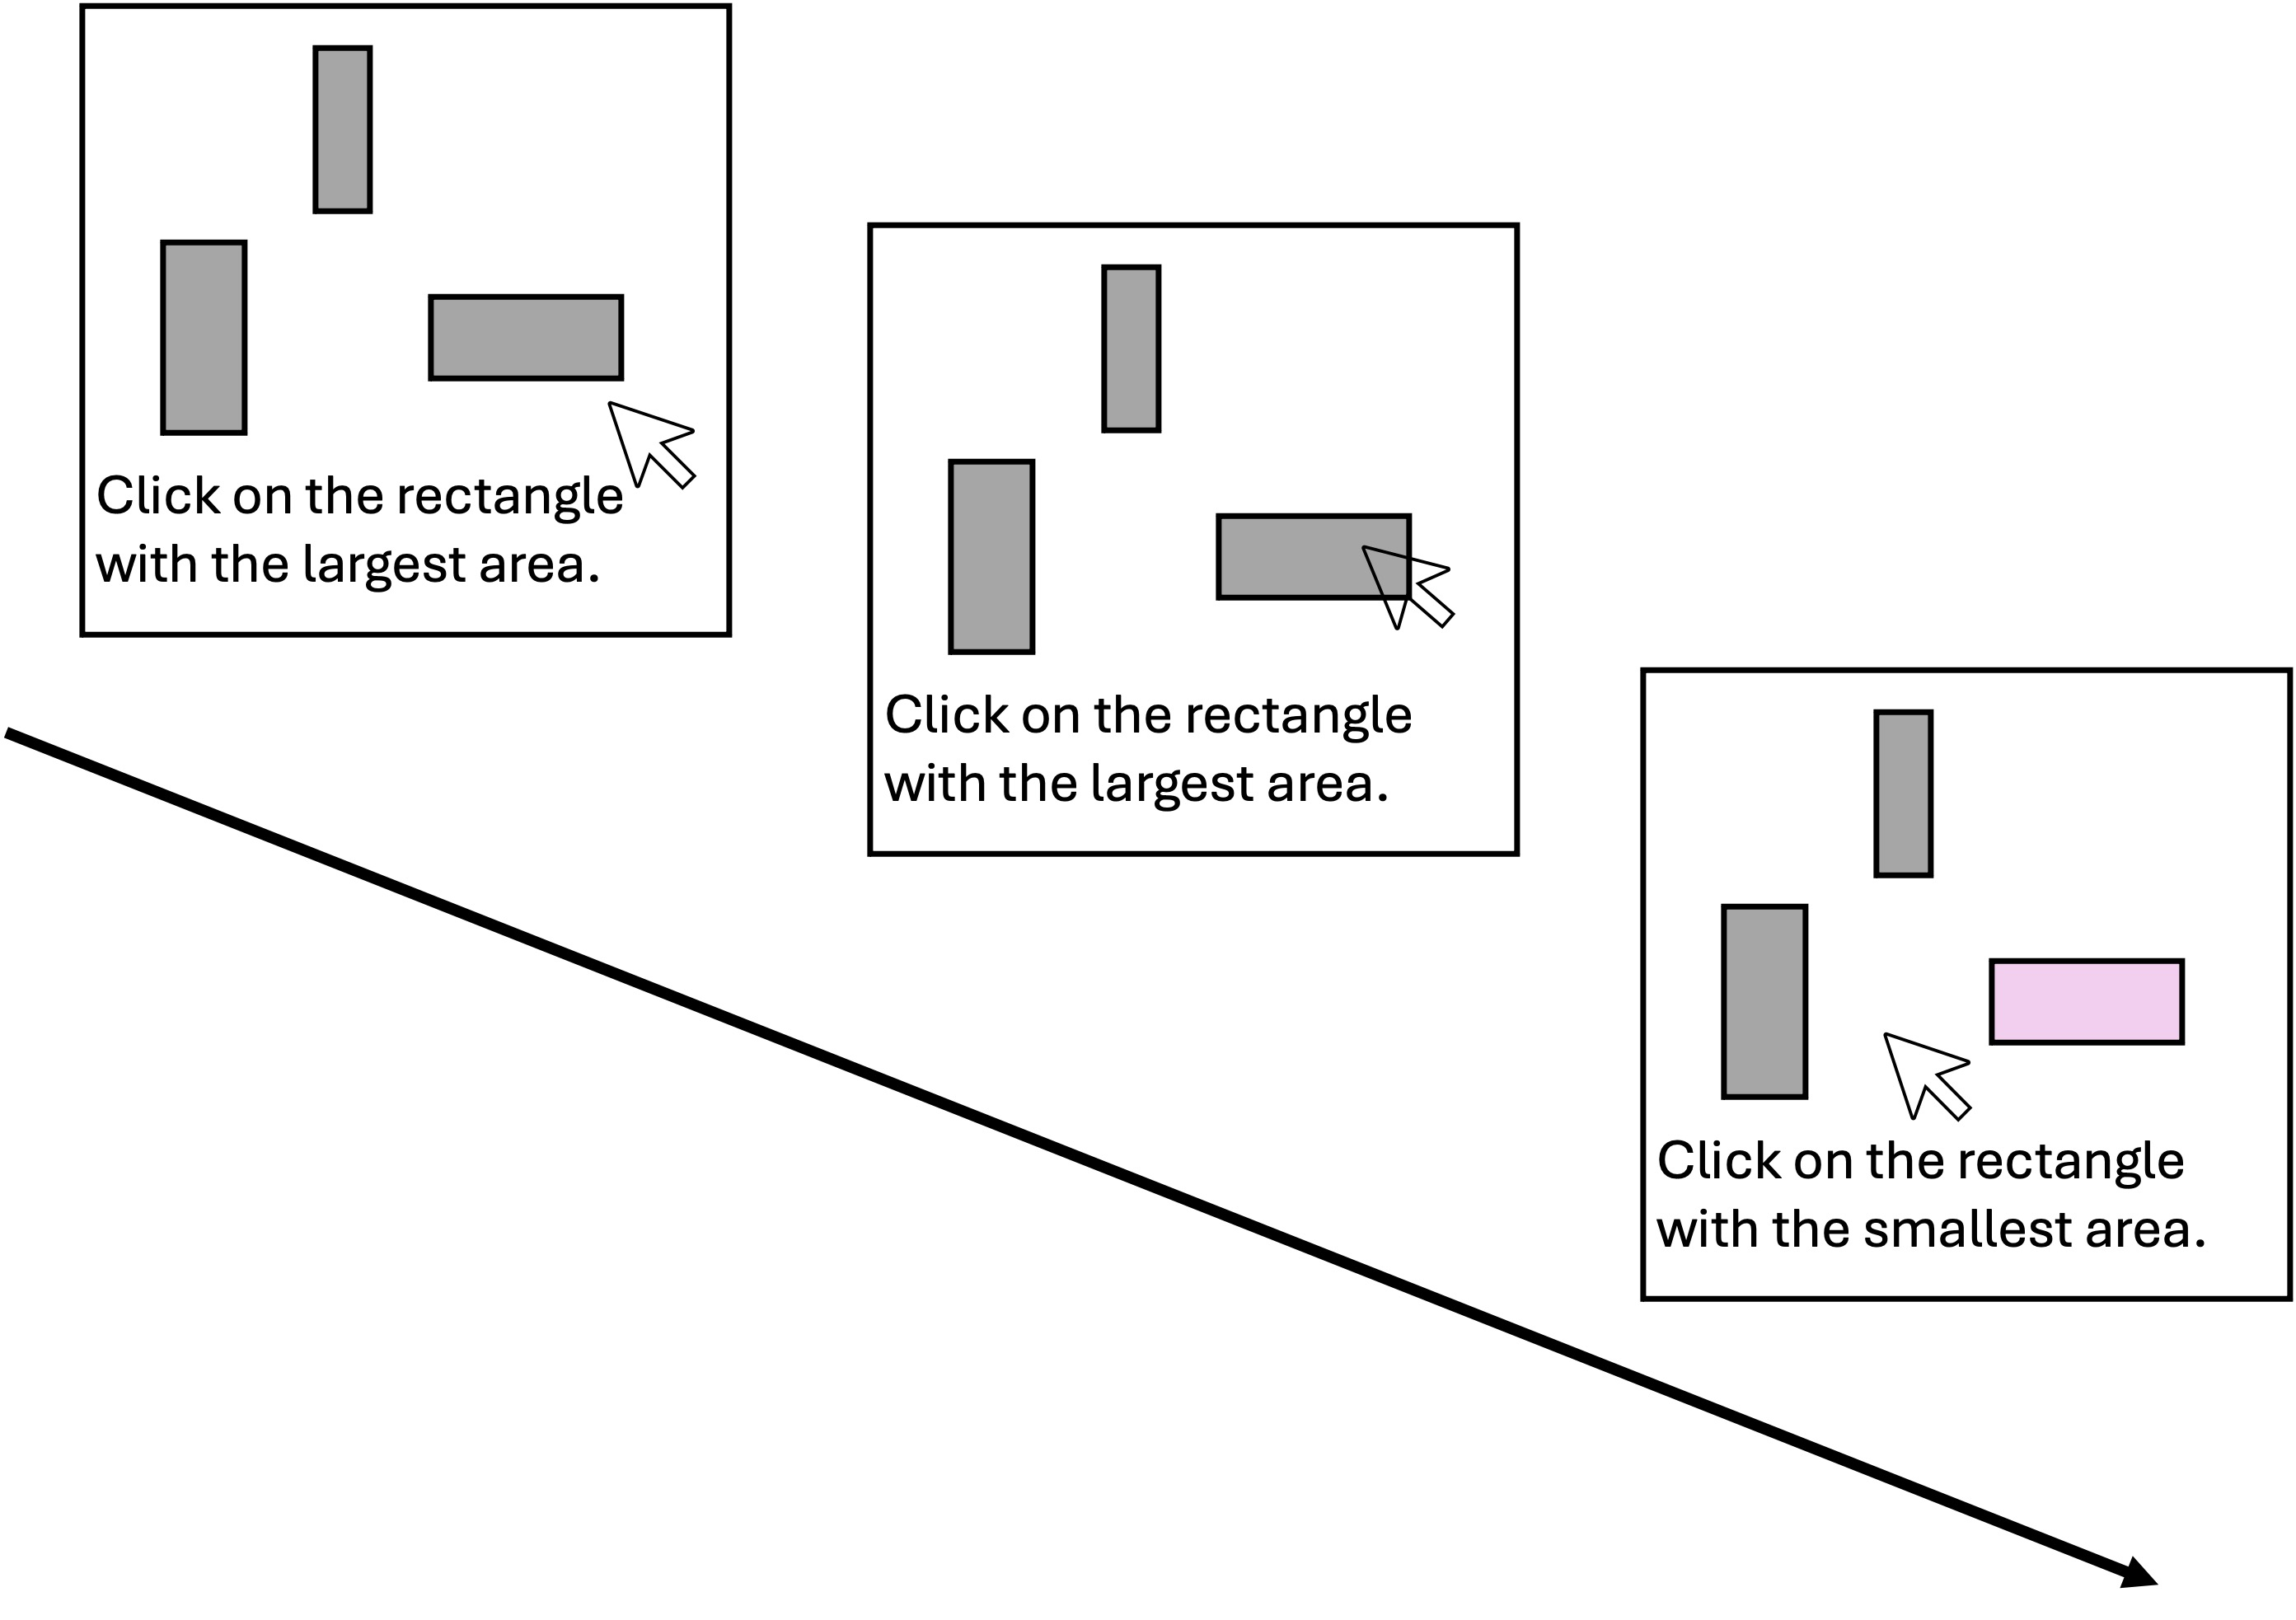
\includegraphics[width=\linewidth]{figures/bw_design_fig.jpg}
   \caption{An example experimental trial for Experiment 3. Note that this is a trial in the best-worst condition.}
   \label{fig:bw_example_trial}
 \end{figure}
 

Stimulus order was randomized on each trial. 

Participants were told their percentage correct of best choices, worst choices, and overall choices at the end of the experiment.

\subsection{Results}

Participants did not meaningfully differ in their choices by condition, so I collapse over condition for all reported analyses.

\subsubsection{Catch Trials.}
Participants performed well on the catch trials. The mean percentage correct for best choices was $97.97\% (SD=14.09)$, and the mean percentage correct for worst choices was $98.26\% (SD=13.09)$. The mean percentage correct for both best and worst choices (i.e., the mean percentage of the trials on which participants were able to correctly identify the largest and smallest rectangles) was $96.98\% (SD=17.12)$. 

\subsubsection{Filler Trials.}
Participants performed worse on the filler trials compared to the catch trials, but still well above chance. The mean percentage correct for best choices was $89.83\% (SD=30.23)$, and the mean percentage correct for worst choices was $88.95\% (SD=13.09)$. The mean percentage correct for both best and worst choices was $96.98\% (SD=17.12)$. 

\subsubsection{Critical Trials.}
I first consider participants choice proportions, conditioned on TDD and choice set. Mean choice proportions for these data are plotted in \ref{fig:bw_mean_choice_by_set}. 

The results show a consistent bias to choose the $w$ (i.e. the option wider than tall) as largest, a finding also shown in Experiments 1 and 2. Participants also (on average) regularly choose the decoy rectangle as smallest, with the exception of the choice set $h,w,d_{w}$ and $TDD=2\%$, where they select the $h$ rectangle as smallest, on average. This can be attributed to the difficulty of the $TDD=2\%$ condition and the overall wide rectangle bias. However, consistent with the predictions of the model, the target is still less likely to be chosen as worst than the competitor, $W(h|{h,w,d_{h}})<W(h|{h,w,d_{w}})$ and $W(w|{h,w,d_{w}})<W(w|{h,w,d_{h}})$, while the competitor option is more likely to be chosen as best, $B(h|{h,w,d_{w}})>B(h|{h,w,d_{h}})$ and $B(w|{h,w,d_{h}})>B(w|{h,w,d_{w}})$. See Appendix XXX for inferential statistics which support these conclusions.

These results are more easily understood by plotting mean target, competitor, and decoy choice proportions across TDD levels, collapsed over choice set. See \ref{fig:bw_mean_choice_collapsed} for these data. First, the best-choice proportions replicate the repulsion effect initially found by \textcite{spektorWhenGoodLooks2018b} and replicated in the current Experiment 2, where the competitor is more likely to be chosen as best at low TDD levels, while the target and competitor are chosen equally often at high TDD levels. Decoy best-choice proportions also decrease systematically with TDD. See Appendix XXX for inferential statistics which support these conclusions. 

Furthermore, the target is always more likely to be chosen as worst, compared to the competitor and decoy, at all TDD levels, $W(T)<W(C)<W(D)$, as predicted by the perceptual model outlined in Chapter 2. This model still cannot predict the null repulsion effect when $TDD=14\%$, as discussed in Chapter 2, which suggests that effect may be due to higher level decision processes.

\begin{figure}
   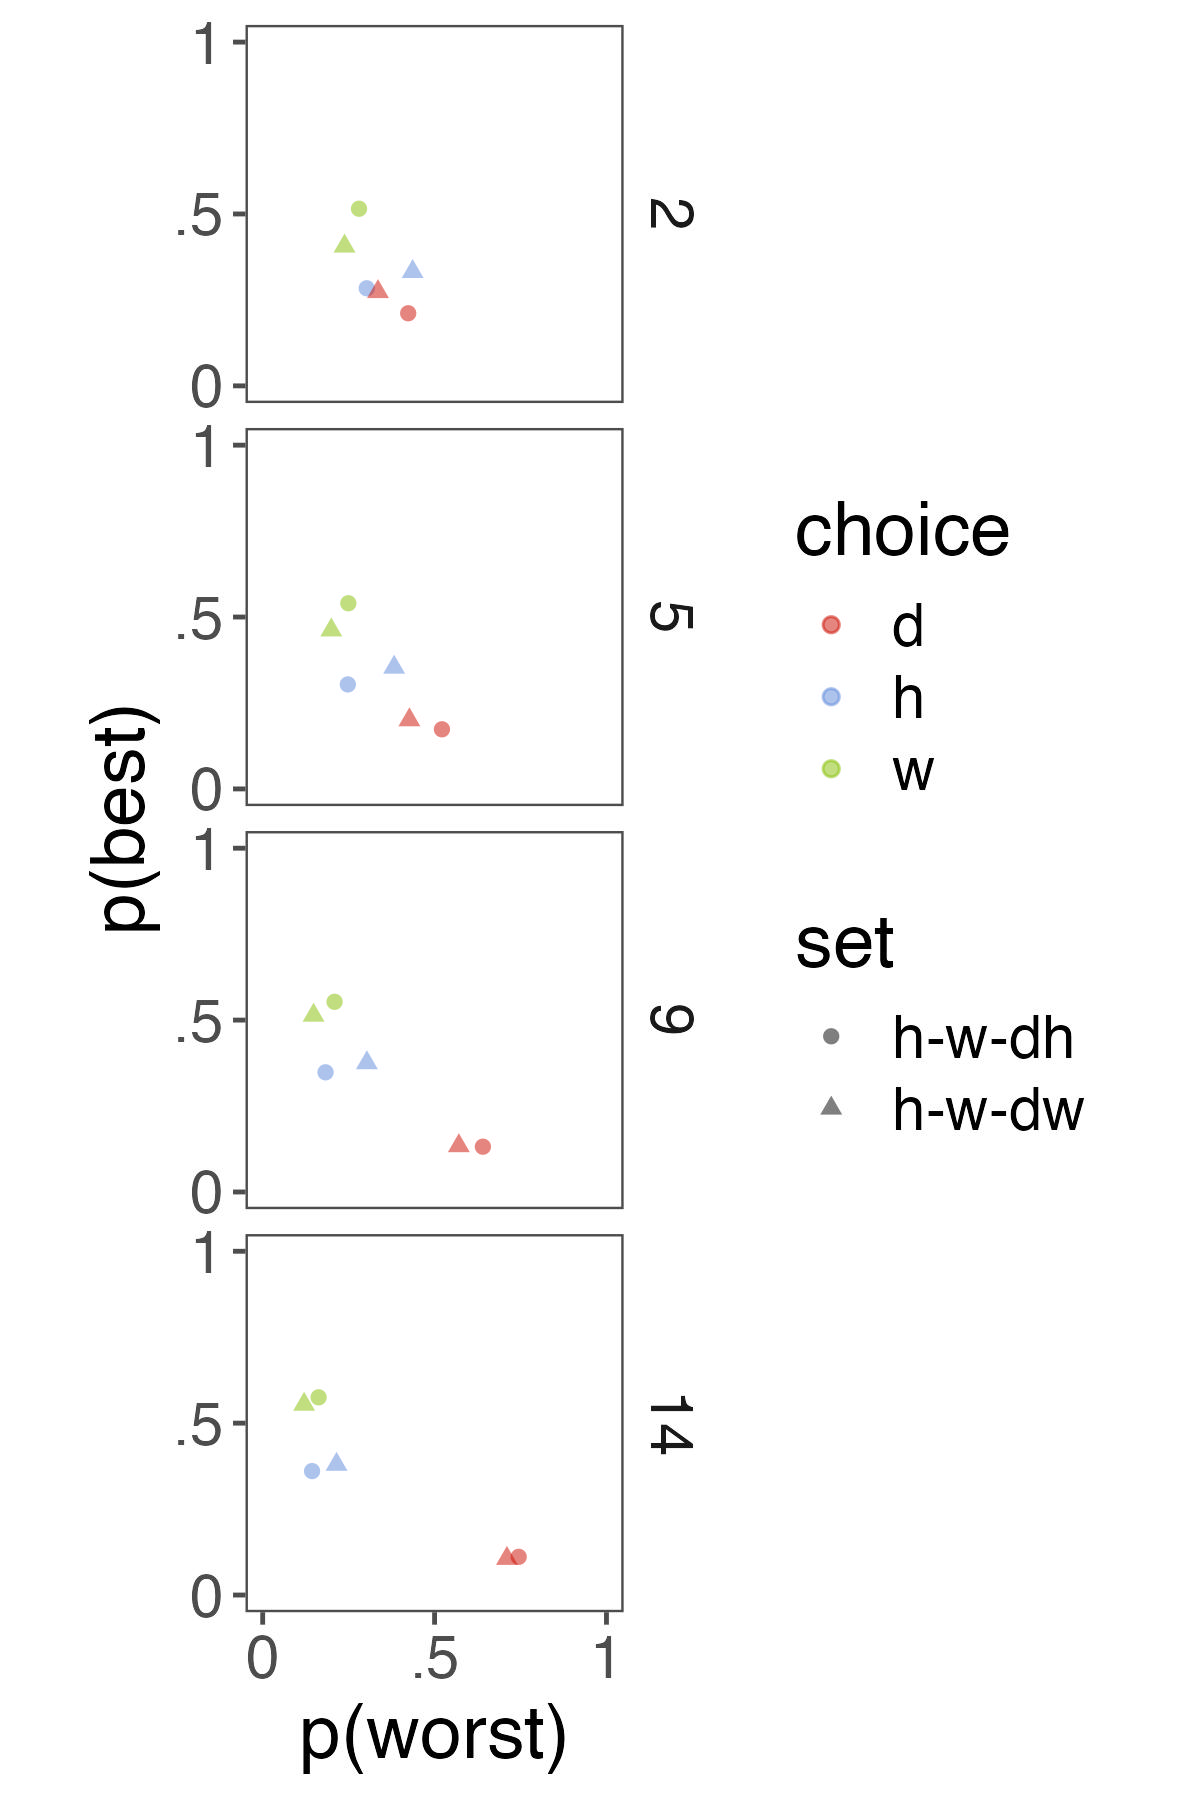
\includegraphics[width=\linewidth]{figures/crit_mean_choice_by_set_dist_labelHW.jpeg}
   \caption{Mean best and worst-choice proportions for the $h$, $w$, and $d$ rectangles, conditioned on TDD (rows) and choice set (shapes).}
   \label{fig:bw_mean_choice_by_set}
 \end{figure}

 \begin{figure}
   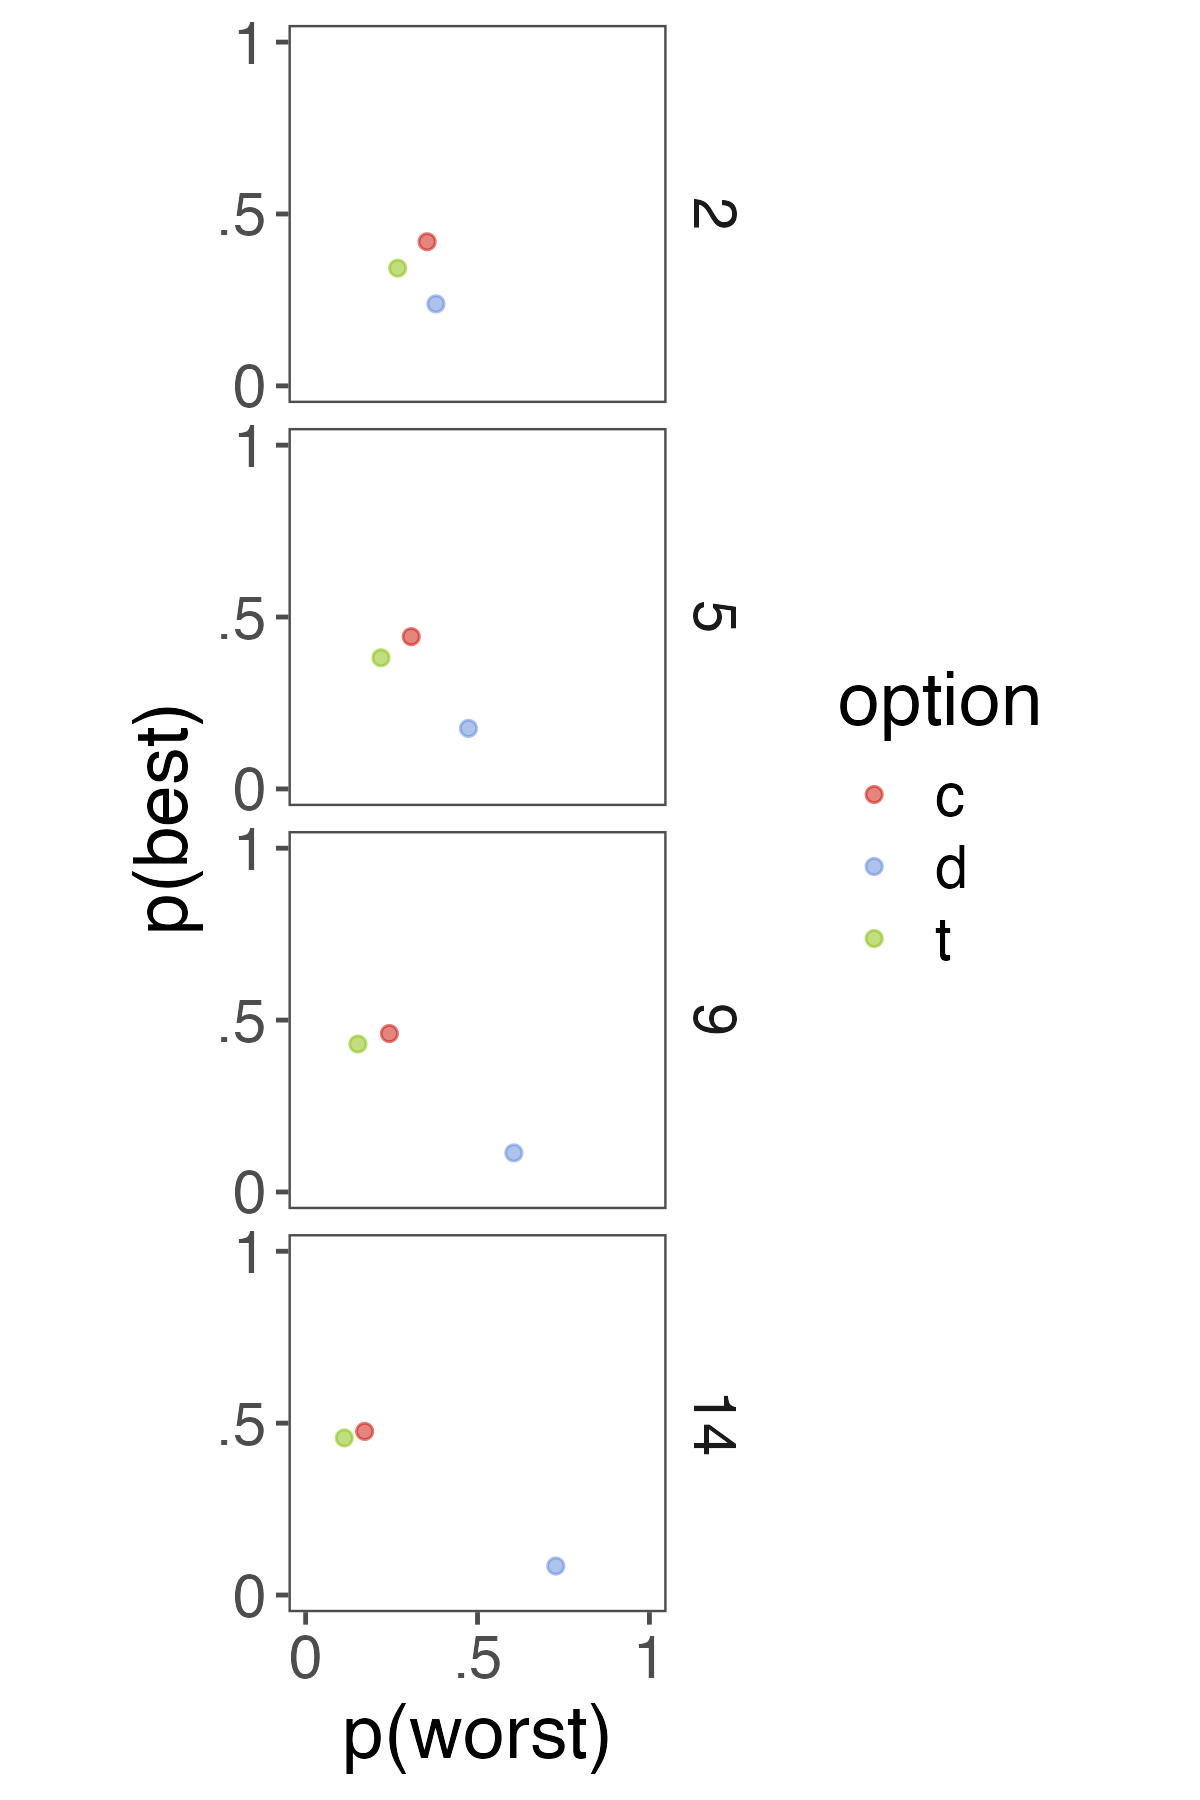
\includegraphics[width=\linewidth]{figures/crit_mean_props_by_dist.jpeg}
   \caption{Mean best and worst-choice proportions for the target, competitor and decoy rectangles, conditioned on TDD (rows).}
   \label{fig:bw_mean_choice_collapsed}
 \end{figure}


\subsubsection{Modeling.}

To analyze the data, I fitted both the maxdiff model and a Dircihlet-multinomial model XXX CITE. The goal of this modeling analysis is to test the ability of a standard best-worst choice model to account for the observed dissociations in the data. The Dirichlet-multinomial is a flexible model that estimates probability distributions around the choice proportions for each participant in each condition. I first consider the maxdiff model.

\subsubsubsection{Maxdiff Modeling}

I first turn to the maxdiff model \parencite{marleyProbabilisticModelsBest2005}, which was outlined in the introduction to this chapter. This equation predicts that the probability of choosing options $x$ and $y$, $x \neq y$ increases monotonically with the difference in their estimated utilities (see \ref{eqn:maxdiff_equation}). This model is the most commonly used (and arguably the simplest) analysis technique for best-worst choice data. I applied this model to the current experiment and show that it is unable to predict the observed dissocations in best-worst choices, even with its best fitting parameters.

I implemented this model as a Bayesian hierarchical model. I show the details of the model fitting procedure, including parameterization, parameter estimates, and all priors in Appendix XXX and focus on the model predictions in the main text. The model predictions for the mean best and worst choices are shown in \ref{fig:maxdiff_collapsed_preds}.

The model clearly mispredicts the data. It predicts that target and competitor are chosen at the nearly the same rate for both best and worst choices. It fares better at predicting decoy choices but is still quantitatively off.

The target-competitor misprediction stems from the fact that the model is predicting the utility of each option through a linear combination of experimental factors, including target/competitor/decoy status. The model could, if the data suggest it, predict that the target has greater utility than the competitor or vice versa. However, because best-choice proportions are positively related to utility and worst-choice proportions are negatively related to utility, the model cannot simultaneously predict $B(C)>B(T)$ and $W(T)<W(C)$. 

I also show participant-level predictions in \ref{fig:maxdiff_sub_preds}. The generally does a poor job at accounting for participant worst-choice proportions, though it performs fair in the best choice 
\begin{figure}
   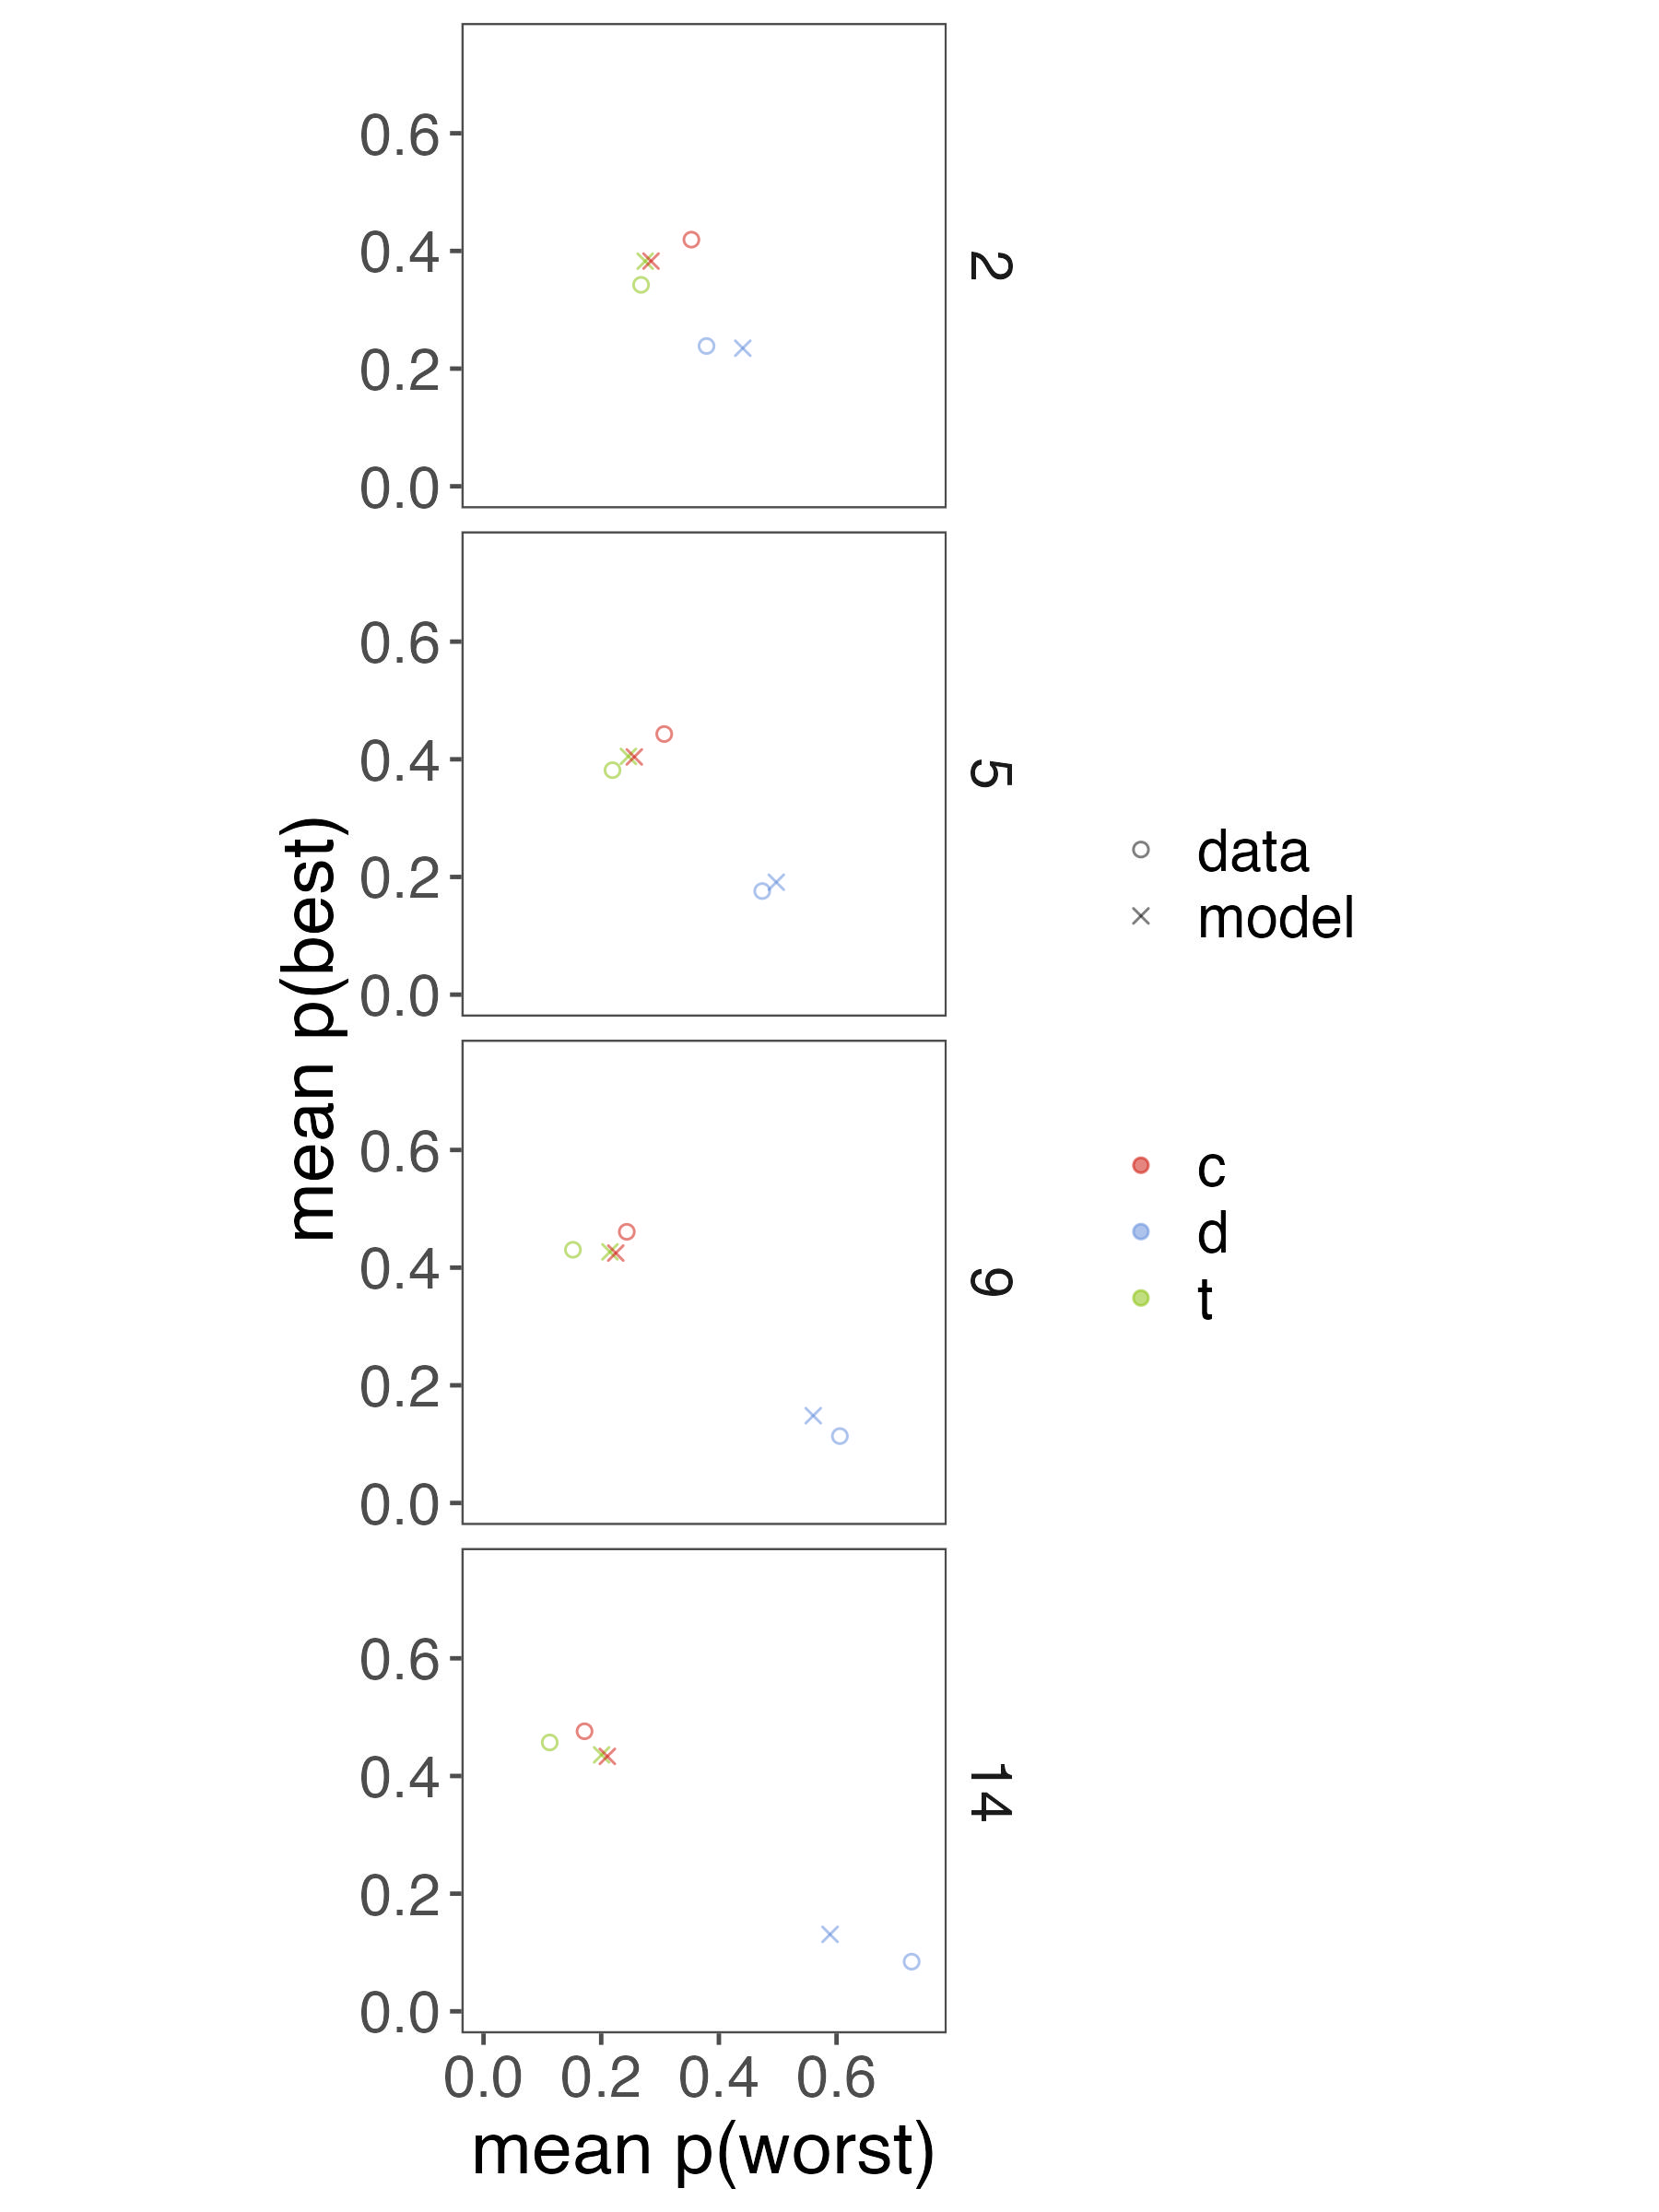
\includegraphics[width=\linewidth]{figures/maxdiff_2_means_model_v_data.jpeg}
   \caption{Maxdiff model predictions for the mean target, competitor, and decoy best-worst choice proportions.}
   \label{fig:maxdiff_collapsed_preds}
\end{figure}

\begin{figure}
   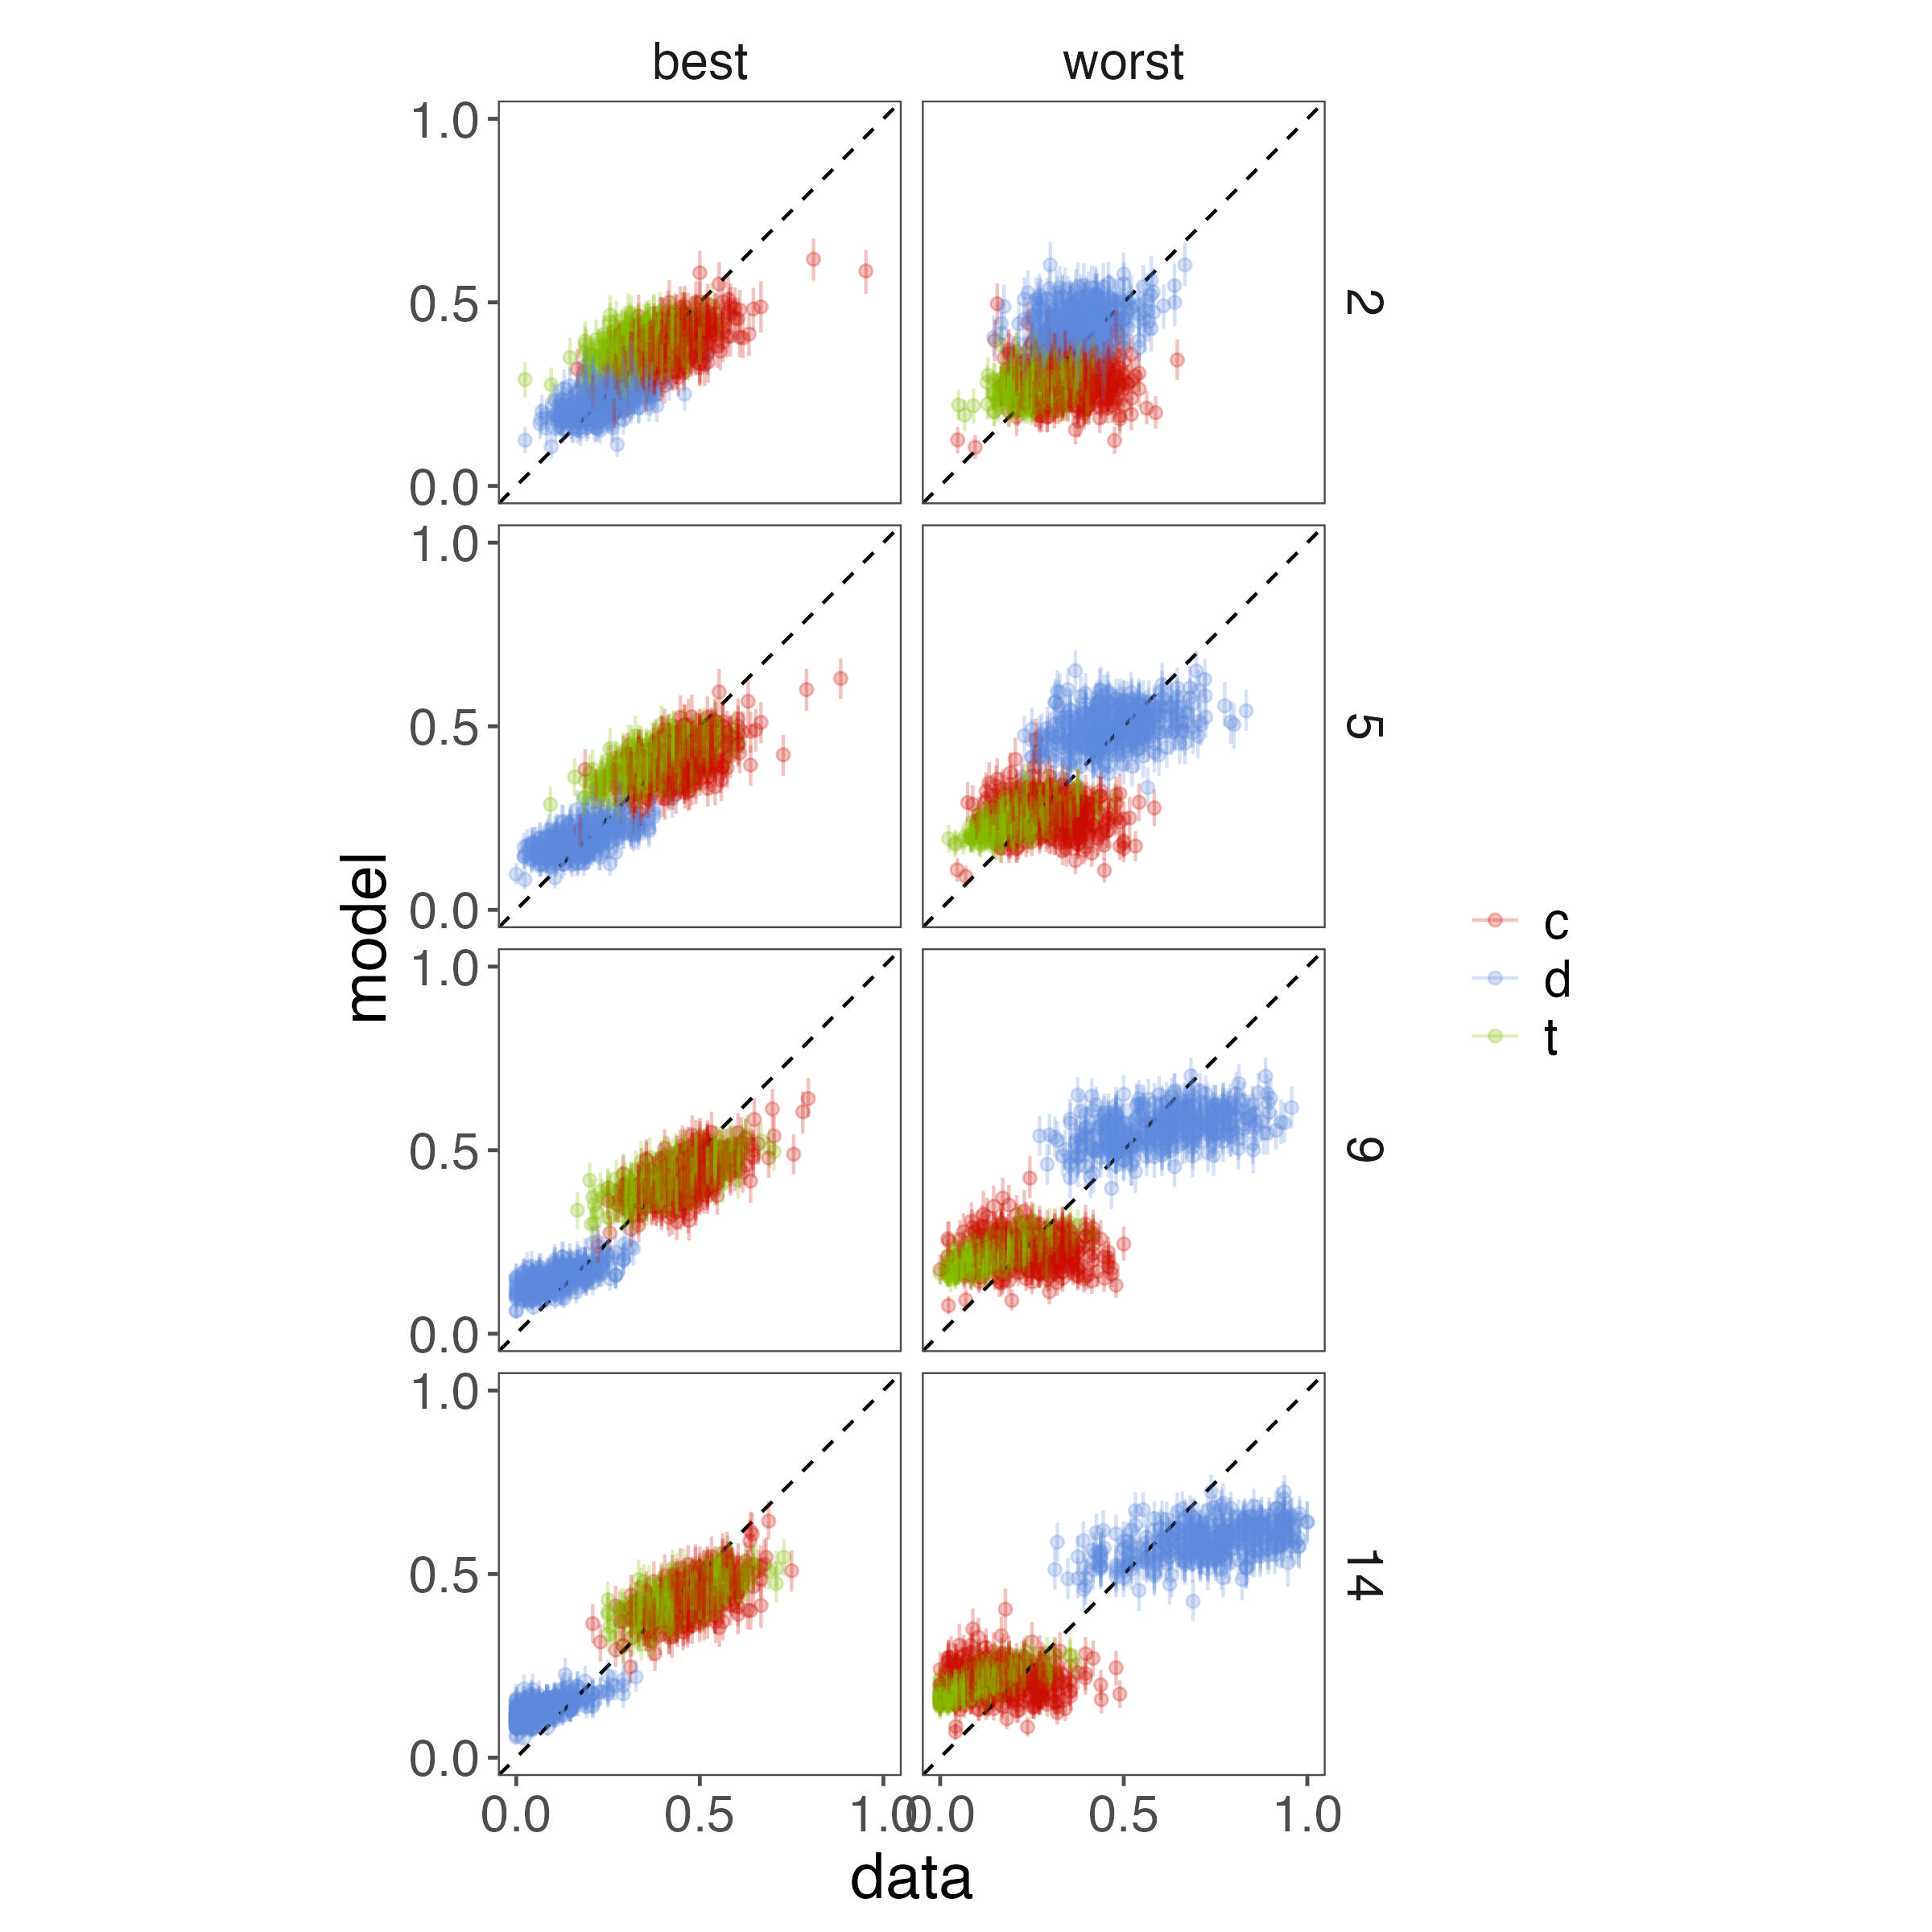
\includegraphics[width=\linewidth]{figures/maxdiff_2_subjectmeans_model_v_data.jpeg}
   \caption{Maxdiff model predictions for the mean target, competitor, and decoy best-worst participant-level choice proportions, conditioned on TDD (rows) and choice type, i.e. best v. worst (columns). Vertical error bars are $95\%$ HDIs.}
   \label{fig:maxdiff_sub_preds}
\end{figure}

\subsubsubsection{Dirichlet-Multinomial Modeling}

